\documentclass{article}
\usepackage[hyphens]{url}
\usepackage{mathtools}
\usepackage{amsmath}
\usepackage{listings}
\usepackage{graphicx}
\usepackage[margin=1in]{geometry}
\usepackage{float}
\floatstyle{boxed}
\restylefloat{figure}
\lstset{breaklines=true}
\begin{document}


\title{CS595 Intro to Web Science, Assignment \#5}
\author{Valentina Neblitt-Jones}
\date{October 17, 2013}
\maketitle

The ``friendship paradox'' (\url{http://en.wikipedia.org/wiki/Friendship_paradox})  says that your friends have more friends than you do. \\

\section*{Question 1}

Determine if the friendship paradox holds for your Facebook account. Create a graph of the number of friends (y-axis) and the friends sorted by number of friends (x-axis). (The friends don't need to be labeled on the x-axis.) Do include yourself in the graph and label yourself accordingly. \\

Compute the mean, standard deviation, and median of the number of friends that your friends have. \\

You can download your network in an XML file by using the NameGenWeb Facebook app:  \\

\url{https://apps.facebook.com/namegenweb} \\

You will need to give this app permission to access your Facebook data. Make sure you select "Friend Count" as an Extended Attribute. When you download the data, download it in the GraphML format. \\

If you do not have a Facebook account, email me and I will send you my GraphML file.

\subsection*{Answer to Question 1}

I discovered when reviewing the GraphML file that some nodes did not contain a Friend Count. I investigated two of those cases and found a difference in summary friends data. Figure \ref{showfriendsprofile} shows a friend whose friend count was in the file and Figure \ref{hidefriendsprofile} shows a friend whose friend count was not in the file. Some of my friends only allow me to see our mutual friends not all of their friends and therefore the application was unable to pull a friend count for those individuals. I have 230 friends, but my report on friend counts only has 208 of those friends' friend counts. This means that 22 of my friends have the mutual friends only setting. I omitted nodes that did not contain a friend count (Figure \ref{nofriendcount}).

\begin{figure}[H]
\centering

\includegraphics[scale=0.75]{q1/showfriendsprofile}
\caption{Showing Friend Count}
\label{showfriendsprofile}
\end{figure}

\begin{figure}[H]
\centering

\includegraphics[scale=0.75]{q1/hidefriendsprofile}
\caption{Hiding Friend Count}
\label{hidefriendsprofile}
\end{figure}

\begin{figure}[H]
\centering
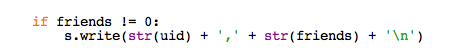
\includegraphics[scale=0.75]{q1/nofriendcount}
\caption{Code that Omits Friends with No Friend Count Available}
\label{nofriendcount}
\end{figure}

%\begin{itemize}
%\item TMZ.com
%\item Sesame Workshop
%\item VT News
%\item Washington City Paper
%\item Library of Congress 
%\end{itemize}

%Figure \ref{inputfile} showed a sample of the input file. It has the md5 and the URI for each link.

%\begin{figure}[H]
%\centering
%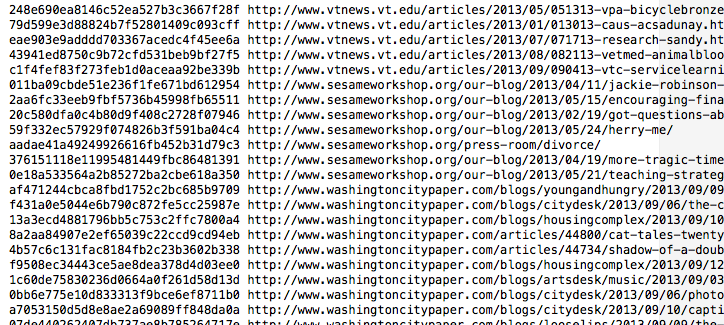
\includegraphics[scale=0.50]{q1/inputfile}
%\caption{Sample of Input File}
%\label{inputfile}
%\end{figure}


\newpage

\section*{Question 2}

Determine if the friendship paradox holds for your Twitter account. Since Twitter is a directed graph, use ``followers'' as value you measure (i.e., ``do your followers have more followers than you?'') \\

Generate the same graph as in question \#1, and calculate the same mean, standard deviation, and median values. \\

For the Twitter 1.1 API to help gather this data, see: \\

\url{https://dev.twitter.com/docs/api/1.1/get/followers/list} \\

If you do not have followers on Twitter (or don't have more than 20), then use my Twitter account ``phonedude\_mln''.

%\begin{table}[!h]
%\centering
%\caption{10 Hits for the term ``shadow'', ranked by TFIDF}
%\begin{tabular}{c c c c}
%\hline
%TFIDF & TF & IDF & URI \\
%\hline
%\hline
%0.150 & 0.014 & 10.680 & http://foo.com \\
%0.085 & 0.008 & 10.680 & http://bar.com \\
%\hline
%\end{tabular}
%\end{table}

\subsection*{Answer to Question 2}


\clearpage

\section*{Extra Credit - LinkedIn (2 points)}

Repeat question \#1, but with your LinkedIn profile.

\subsection*{Answer to Extra Credit - LinkedIn}

\clearpage

\section*{Extra Credit - Twitter (1 point)}

Repeat question \#2, but change ``followers'' to ``following''? In other words, are the people I am following following more people?

\subsection*{Answer to Extra Credit - Twitter}

\clearpage

\section*{Resources}

\begin{itemize}
\item Grosfield, Troy. Parsing XML with Python using ElementTree. \url{http://blog.troygrosfield.com/2010/12/18/parsing-xml-with-python-using-elementtree/}
\item McCown, Frank. Producing Simple Graphs with R. \url{http://www.harding.edu/fmccown/r/}
\item Poulson, Barton. R Statistics Essential Training. \url{http://www.lynda.com/course20/R-tutorials/R-Statistics-Essential-Training/142447-2.html}
\item Python.org. The ElementTree XML API. \url{http://docs.python.org/3.3/library/xml.etree.elementtree.html}
\item Seminar for Statistics. R Documentation: Arithmetic Mean. \url{http://stat.ethz.ch/R-manual/R-devel/library/base/html/mean.html}
\item Seminar for Statistics. R Documentation: Concatenate Strings. \url{http://stat.ethz.ch/R-manual/R-devel/library/base/html/paste.html}
\item Seminar for Statistics. R Documentation: Median Value. \url{http://stat.ethz.ch/R-manual/R-patched/library/stats/html/median.html}
\item Seminar for Statistics. R Documentation: Standard Deviation. \url{http://stat.ethz.ch/R-manual/R-patched/library/stats/html/sd.html}
\item Stack Overflow. Change colors or particular bars in a bar chart. \url{http://stackoverflow.com/questions/13112974/change-colours-of-particular-bars-in-a-bar-chart}
\item Stack Overflow. How do you print to stderr in R? \url{http://stackoverflow.com/questions/1109017/how-do-you-print-to-stderr-in-r}
\item Stack Overflow. Understanding the Order() function in R. \url{http://stackoverflow.com/questions/2315601/understanding-the-order-function-in-r}
\item Twitter Developers Documentation. GET followers/list. \url{https://dev.twitter.com/docs/api/1.1/get/followers/list}
\end{itemize}

\end{document}